% ============================================================================
% ANEXO 3: COMPARA\c{C}\~AO ENTRE M\'ETODOS DE CARACTERIZA\c{C}\~AO
% ============================================================================

\section{Compara\c{c}\~ao entre M\'etodos de Caracteriza\c{c}\~ao para Forma\c{c}\~ao de Material Particulado}
\label{anexo:comparacao-metodos}

Este anexo apresenta a compara\c{c}\~ao dos resultados de impacto direto obtidos no OpenLCA utilizando diferentes m\'etodos de caracteriza\c{c}\~ao para forma\c{c}\~ao de material particulado (PM). A an\'alise foi conduzida com o invent\'ario de produ\c{c}\~ao de soja dispon\'ivel no SICV Brasil (IBICT), com dados regionalizados para 11 estados brasileiros.

% ============================================================================
\subsection{Delineamento da compara\c{c}\~ao}
% ============================================================================

\subsubsection{Invent\'ario utilizado}

O invent\'ario de produ\c{c}\~ao de soja foi obtido do Sistema de Invent\'ario do Ciclo de Vida do IBICT\footnote{\url{https://sicv.acv.ibict.br/showProcess.xhtml?uuid=a7608c64-0d99-5c01-9dd9-001f97b4d8bb&version=03.01.000&stock=default}}, contemplando dados regionalizados para os estados de Bahia (BA), Goi\'as (GO), Maranh\~ao (MA), Minas Gerais (MG), Mato Grosso do Sul (MS), Mato Grosso (MT), Piau\'i (PI), Paran\'a (PR), Rio Grande do Sul (RS), S\~ao Paulo (SP) e Tocantins (TO).

Como os fatores de caracteriza\c{c}\~ao do RAICV-BR-PM s\~ao regionalizados por estado e Giusti (2025) n\~ao calculou um FC global, realizou-se somente a an\'alise de impactos diretos, sem ciclo de vida completo.

\subsubsection{M\'etodos comparados}

Cinco m\'etodos de caracteriza\c{c}\~ao para forma\c{c}\~ao de material particulado foram comparados:

\begin{table}[H]
\centering
\caption{M\'etodos de caracteriza\c{c}\~ao comparados}
\label{tab:metodos-comparados}
\begin{tabular}{llll}
\toprule
\textbf{M\'etodo} & \textbf{Escopo} & \textbf{Tipo de FC} & \textbf{Refer\^encia} \\
\midrule
RAICV-BR  & Brasil (27 estados) & Regionalizado & Giusti (2025) \\
GLAM-BR   & Brasil (agregado)   & Nacional      & Fantke et al. (2019) \\
GLAM-GLO  & Global              & Global        & Fantke et al. (2019) \\
OBER-BR   & Brasil (27 estados) & Regionalizado & Oberschelp et al. (2020) \\
ReCiPe    & Global              & Global        & Huijbregts et al. (2017) \\
\bottomrule
\end{tabular}
\end{table}

Cada m\'etodo foi convertido em pacote JSON-LD e importado no OpenLCA utilizando a ferramenta \texttt{olca-cf-converter}. Os impactos diretos foram calculados para as quatro subst\^ancias precursoras de material particulado: am\^onia (NH\textsubscript{3}), \'oxidos de nitrog\^enio (NO\textsubscript{x}), material particulado fino (PM\textsubscript{2,5}) e di\'oxido de enxofre (SO\textsubscript{2}).

\subsubsection{M\'etrica de compara\c{c}\~ao}

A diverg\^encia entre cada m\'etodo alternativo e o RAICV-BR (refer\^encia) foi quantificada pelo sMAPE (\textit{Symmetric Mean Absolute Percentage Error}). Essa m\'etrica varia de 0\% (concord\^ancia perfeita) a 200\% (diverg\^encia m\'axima), sendo sim\'etrica em rela\c{c}\~ao a sobre e subestima\c{c}\~ao.

% ============================================================================
\subsection{Resultados}
% ============================================================================

\subsubsection{Concord\^ancia geral por m\'etodo}

A Tabela~\ref{tab:smape-medio} apresenta o sMAPE m\'edio por m\'etodo e subst\^ancia. Valores menores indicam maior proximidade com o RAICV-BR.

\begin{table}[H]
\centering
\caption{sMAPE m\'edio (\%) por m\'etodo e subst\^ancia, em rela\c{c}\~ao ao RAICV-BR}
\label{tab:smape-medio}
\begin{tabular}{lrrrrr}
\toprule
\textbf{M\'etodo} & \textbf{NH\textsubscript{3}} & \textbf{NO\textsubscript{x}} & \textbf{PM\textsubscript{2,5}} & \textbf{SO\textsubscript{2}} & \textbf{M\'edia} \\
\midrule
ReCiPe   & 109,4 &  64,3 &  67,4 &  89,1 & \textbf{82,6} \\
GLAM-GLO & 105,8 &  59,8 &  69,4 & 129,7 & \textbf{91,2} \\
OBER-BR  &  92,9 & 138,5 & 129,0 & 183,9 & \textbf{136,1} \\
GLAM-BR  & 121,0 & 142,7 & 124,9 & 183,9 & \textbf{143,1} \\
\bottomrule
\end{tabular}
\end{table}

O ReCiPe apresentou a maior concord\^ancia geral com o RAICV-BR (sMAPE m\'edio = 82,6\%), seguido pelo GLAM-GLO (91,2\%). Os m\'etodos regionalizados para o Brasil --- Oberschelp (136,1\%) e GLAM-BR (143,1\%) --- mostraram diverg\^encias maiores.

Esse resultado pode parecer contradit\'orio: seria de esperar que m\'etodos regionalizados para o Brasil concordassem mais com o RAICV-BR. Contudo, embora todos sejam ``regionalizados'', cada modelo parte de premissas de modelagem atmosf\'erica, resolu\c{c}\~oes espaciais e fun\c{c}\~oes dose-resposta distintas. O RAICV-BR utiliza modelagem espec\'ifica para o territ\'orio brasileiro (Giusti, 2025), com condi\c{c}\~oes meteorol\'ogicas e demogr\'aficas distintas das adotadas pelo GLAM e pelo Oberschelp.

A Figura~\ref{fig:boxplot} apresenta a distribui\c{c}\~ao do sMAPE por m\'etodo.

\begin{figure}[H]
\centering
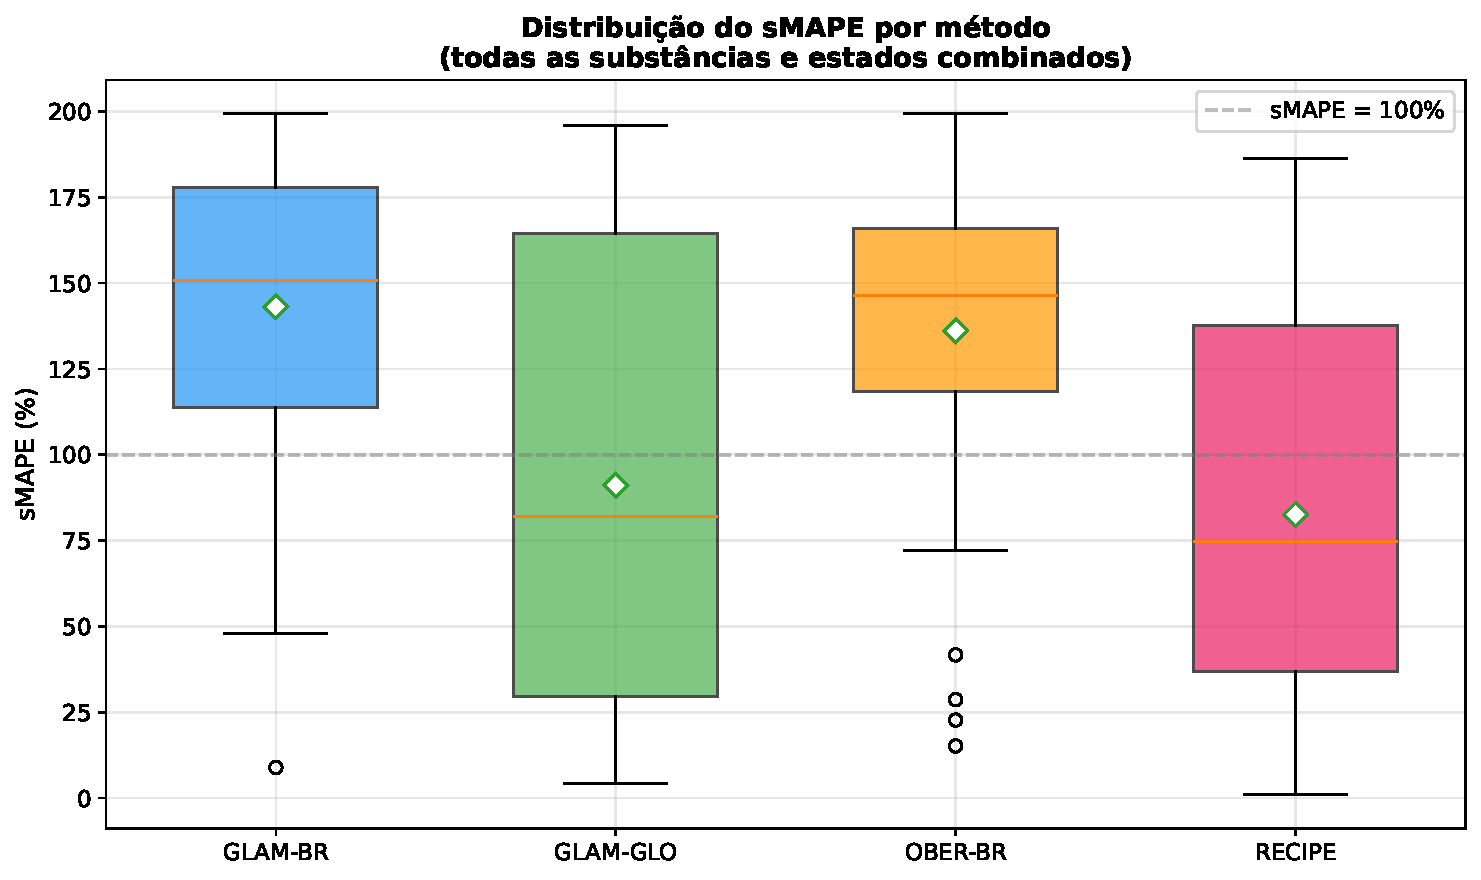
\includegraphics[width=0.85\textwidth]{figuras/fig2-boxplot-metodos.pdf}
\caption{Distribui\c{c}\~ao do sMAPE por m\'etodo (todas as subst\^ancias e estados combinados). O losango branco indica a m\'edia; a linha horizontal indica a mediana. A linha tracejada marca sMAPE = 100\%.}
\label{fig:boxplot}
\end{figure}

\subsubsection{An\'alise por subst\^ancia}

A Figura~\ref{fig:heatmap} apresenta o sMAPE desagregado por subst\^ancia, estado e m\'etodo. Cores vermelhas indicam alta diverg\^encia com o RAICV-BR; cores verdes indicam alta concord\^ancia.

\begin{figure}[H]
\centering
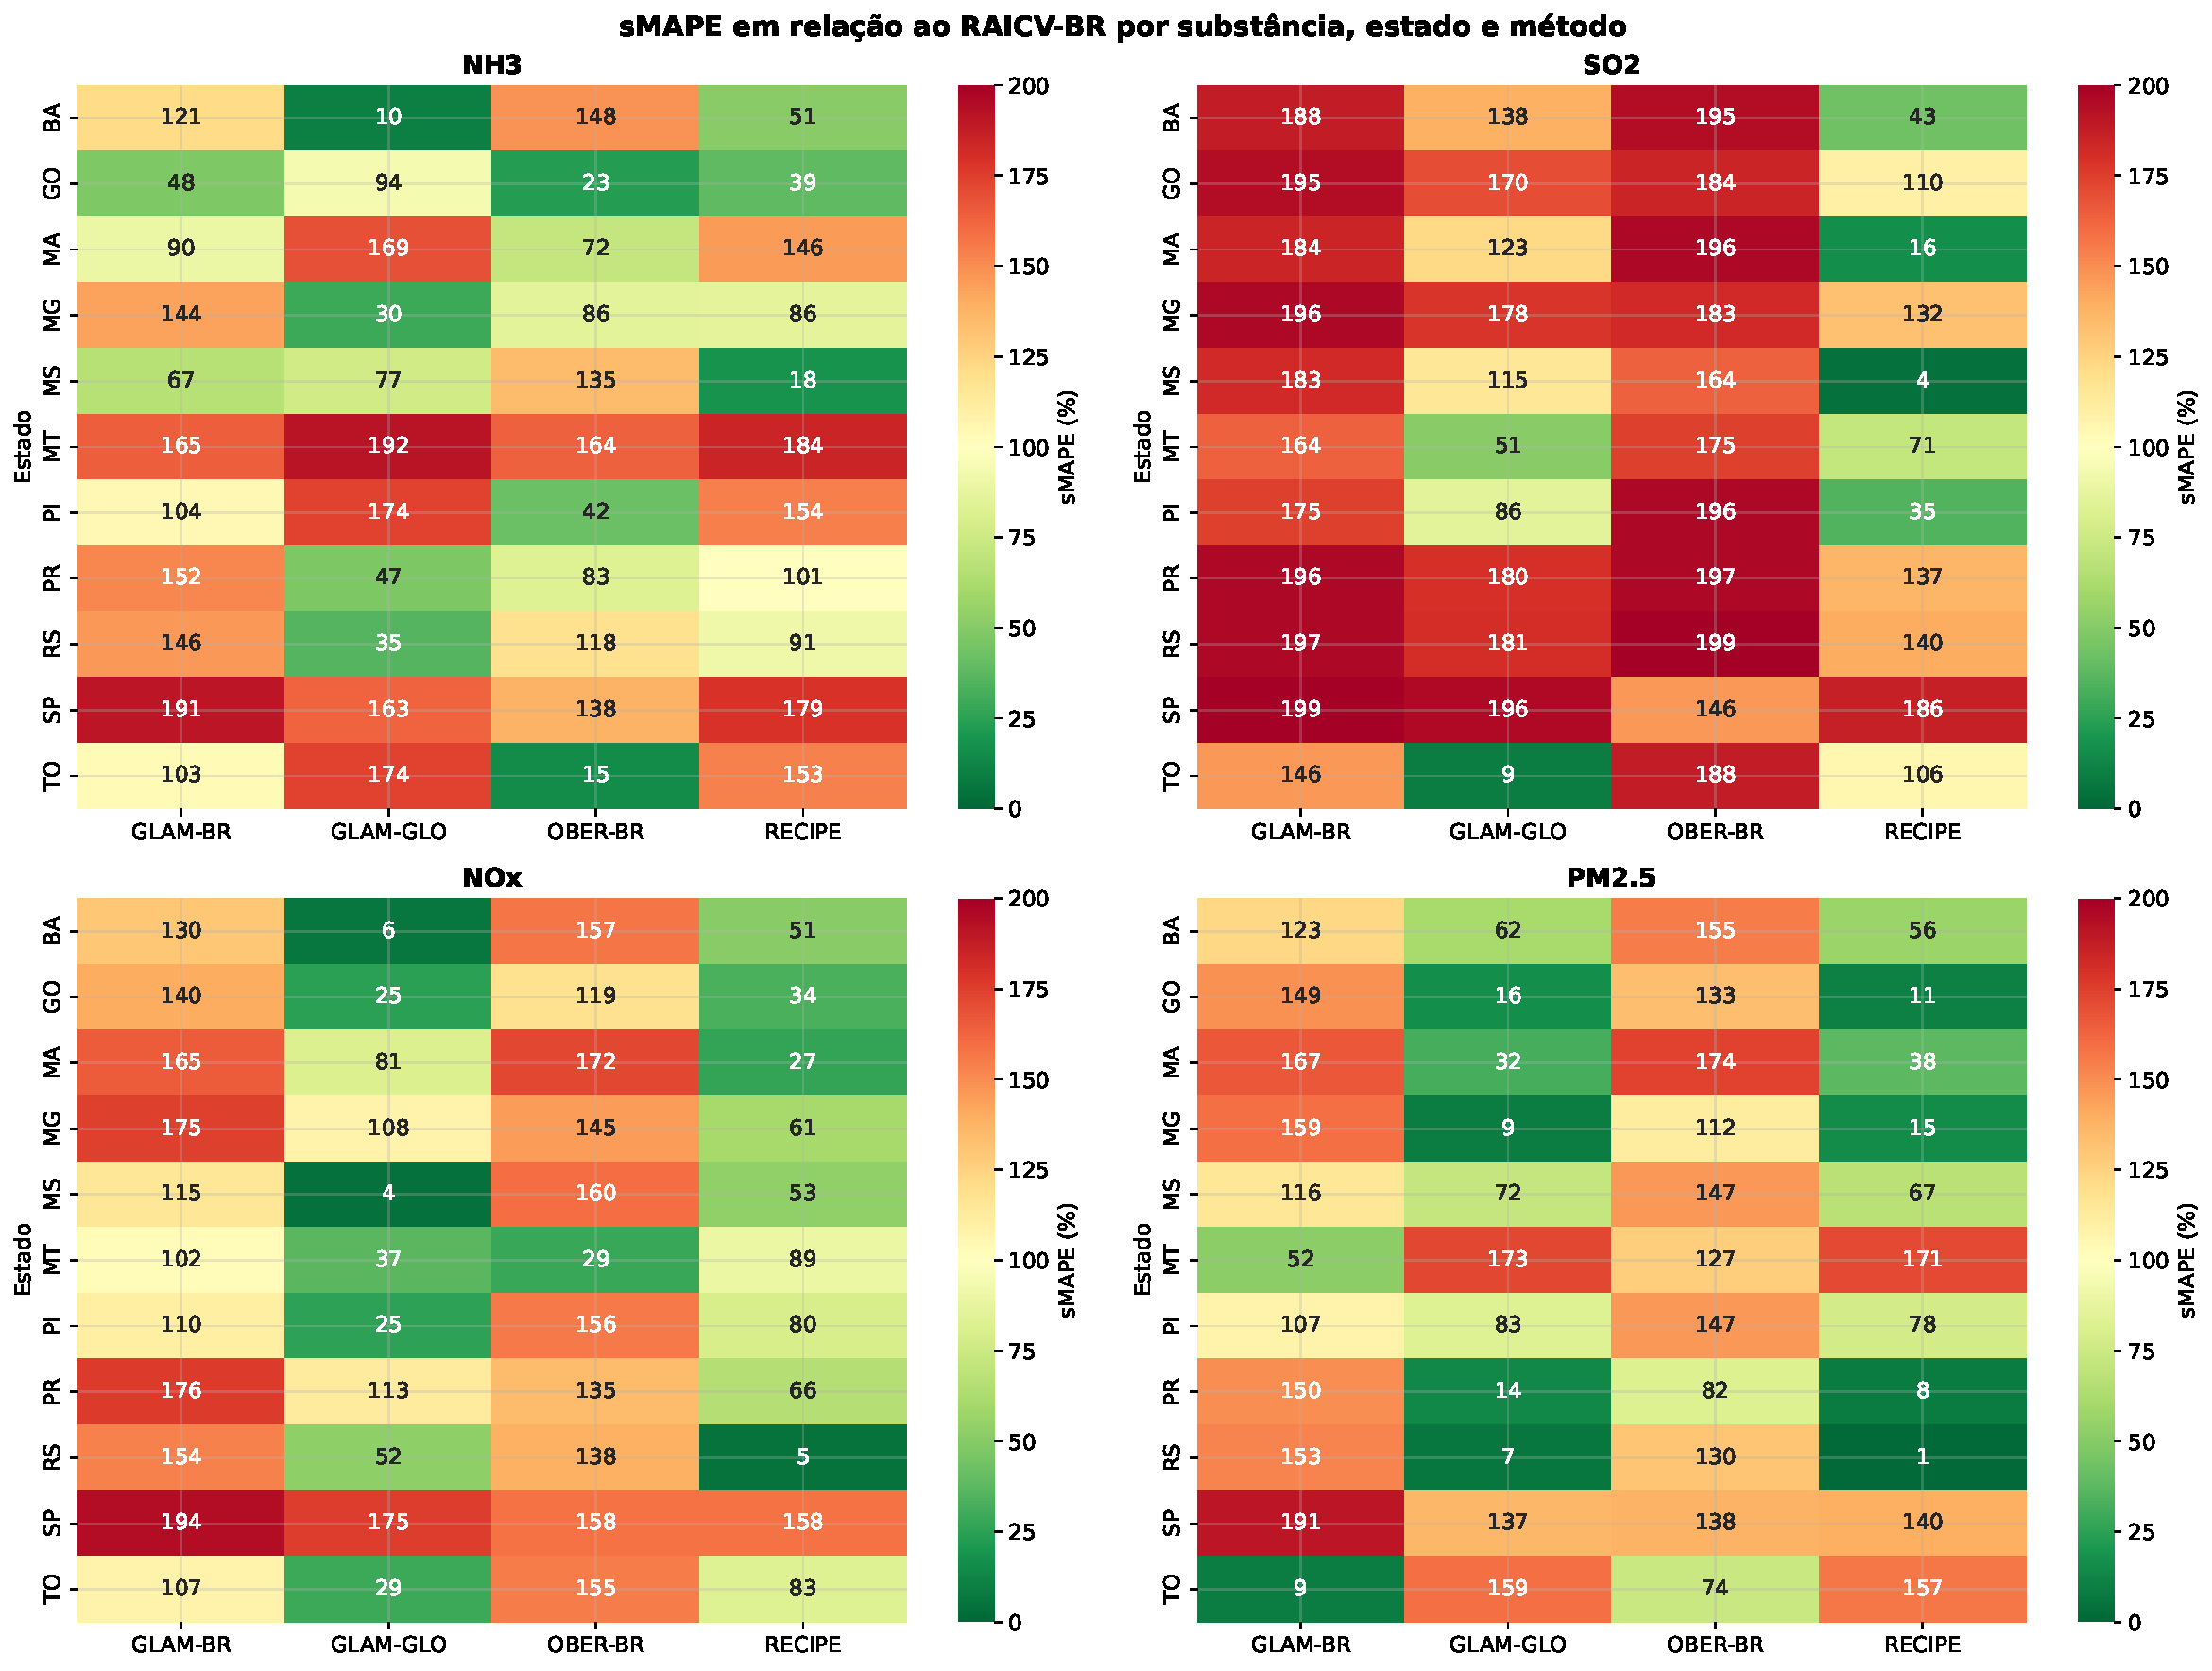
\includegraphics[width=\textwidth]{figuras/fig1-heatmap-smape-4substancias.pdf}
\caption{sMAPE (\%) em rela\c{c}\~ao ao RAICV-BR por subst\^ancia, estado e m\'etodo. Valores anotados em cada c\'elula.}
\label{fig:heatmap}
\end{figure}

A signific\^ancia das diferen\c{c}as entre m\'etodos foi testada pelo teste n\~ao param\'etrico de Kruskal-Wallis, adequado para amostras pequenas com distribui\c{c}\~oes n\~ao-normais:

\begin{table}[H]
\centering
\caption{Teste de Kruskal-Wallis para diferen\c{c}as entre m\'etodos por subst\^ancia}
\label{tab:kruskal}
\begin{tabular}{lrrl}
\toprule
\textbf{Subst\^ancia} & \textbf{H} & \textbf{p-valor} & \textbf{Significativo ($\alpha$=0,05)?} \\
\midrule
NH\textsubscript{3}    &  1,78 & 0,620   & N\~ao \\
NO\textsubscript{x}    & 19,32 & 0,0002  & \textbf{Sim} \\
PM\textsubscript{2,5}  &  8,09 & 0,044   & \textbf{Sim} \\
SO\textsubscript{2}    & 22,65 & $<$0,0001 & \textbf{Sim} \\
\bottomrule
\end{tabular}
\end{table}

Para tr\^es das quatro subst\^ancias (NO\textsubscript{x}, PM\textsubscript{2,5} e SO\textsubscript{2}), a escolha do m\'etodo de caracteriza\c{c}\~ao impacta de forma estatisticamente significativa os resultados de impacto. Somente para a am\^onia as diferen\c{c}as n\~ao alcan\c{c}aram signific\^ancia, sugerindo que os m\'etodos tendem a convergir para essa subst\^ancia --- possivelmente porque o transporte e a forma\c{c}\~ao de particulado secund\'ario a partir de NH\textsubscript{3} seguem padr\~oes mais uniformes no territ\'orio brasileiro.

\subsubsection{An\'alise por estado}

A Tabela~\ref{tab:smape-estado} apresenta o sMAPE m\'edio por estado, revelando quais regi\~oes s\~ao mais sens\'iveis \`a escolha do m\'etodo.

\begin{table}[H]
\centering
\caption{sMAPE m\'edio por estado (todos os m\'etodos e subst\^ancias combinados)}
\label{tab:smape-estado}
\begin{tabular}{lrrrr}
\toprule
\textbf{Estado} & \textbf{M\'edia (\%)} & \textbf{DP} & \textbf{M\'in (\%)} & \textbf{M\'ax (\%)} \\
\midrule
SP & 168,1 & 23,6  & 136,6 & 199,3 \\
MT & 121,5 & 58,7  &  28,7 & 191,6 \\
MA & 115,8 & 63,9  &  15,9 & 196,2 \\
PR & 114,8 & 60,9  &   8,2 & 196,7 \\
MG & 113,6 & 61,0  &   9,2 & 196,2 \\
PI & 109,4 & 52,9  &  25,2 & 196,5 \\
RS & 109,3 & 68,6  &   1,1 & 199,3 \\
TO & 104,3 & 61,9  &   8,8 & 188,1 \\
BA & 102,3 & 61,6  &   6,4 & 194,5 \\
MS &  93,6 & 56,9  &   4,3 & 182,6 \\
GO &  93,0 & 64,9  &  10,5 & 194,5 \\
\bottomrule
\end{tabular}
\end{table}

S\~ao Paulo destaca-se com o maior sMAPE m\'edio (168,1\%) e o menor desvio-padr\~ao (23,6\%), indicando que \textit{todos} os m\'etodos alternativos divergem fortemente do RAICV-BR para esse estado. Essa observa\c{c}\~ao \'e coerente com as particularidades de SP: a maior regi\~ao metropolitana do hemisf\'erio sul possui qu\'imica atmosf\'erica dominada por intera\c{c}\~oes complexas entre emiss\~oes veiculares, industriais e agr\'icolas que m\'etodos gen\'ericos n\~ao capturam adequadamente.

Em contraste, Goi\'as e Mato Grosso do Sul apresentam os menores sMAPEs m\'edios ($\sim$93\%), sugerindo que, para estados com perfil agr\'icola predominante e menor densidade urbana, os m\'etodos tendem a convergir.

O perfil espacial da diverg\^encia por subst\^ancia e estado \'e apresentado na Figura~\ref{fig:radar}.

\begin{figure}[H]
\centering
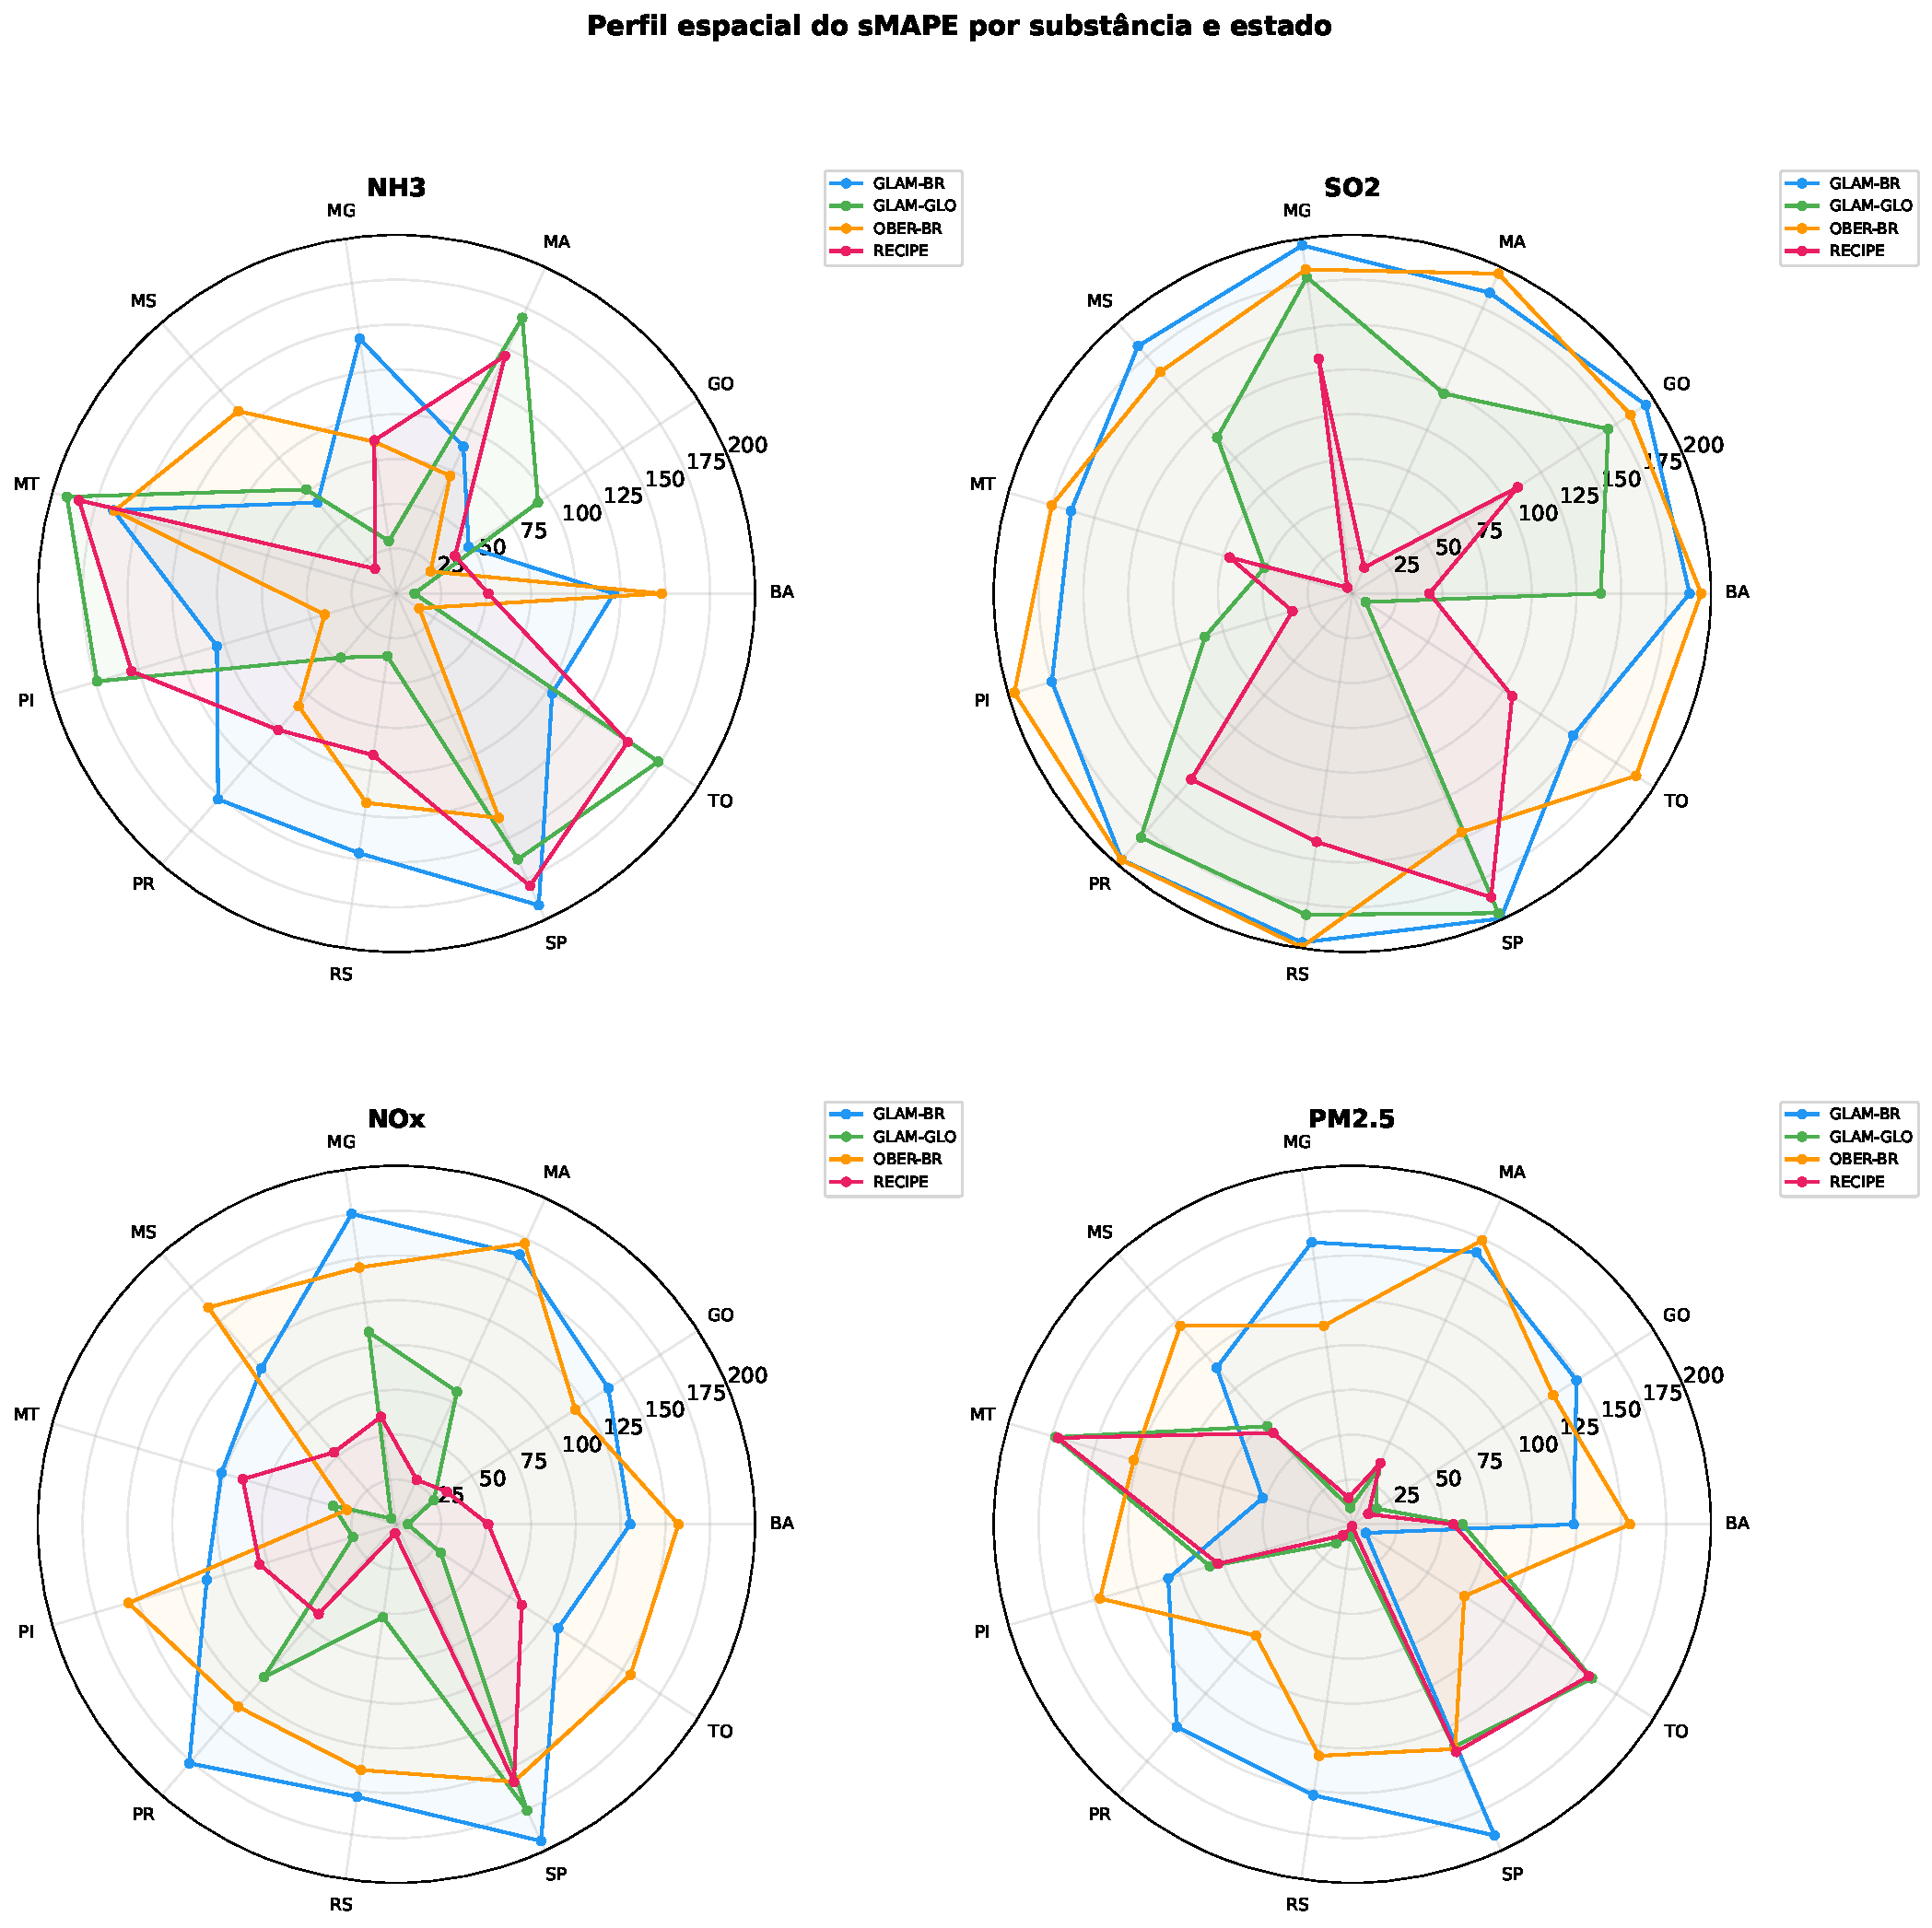
\includegraphics[width=\textwidth]{figuras/fig3-radar-estados.pdf}
\caption{Perfil espacial do sMAPE por subst\^ancia e estado. Cada eixo representa um estado; a dist\^ancia do centro indica o sMAPE (\%).}
\label{fig:radar}
\end{figure}

\subsubsection{M\'etodo mais pr\'oximo do RAICV-BR por contexto}

Das 44 combina\c{c}\~oes poss\'iveis (11 estados $\times$ 4 subst\^ancias), analisou-se qual m\'etodo alternativo apresenta menor sMAPE em cada caso (Tabela~\ref{tab:vitorias} e Figura~\ref{fig:vitorias}).

\begin{table}[H]
\centering
\caption{Contagem de ``vit\'orias'' --- m\'etodo mais pr\'oximo do RAICV-BR}
\label{tab:vitorias}
\begin{tabular}{lrr}
\toprule
\textbf{M\'etodo} & \textbf{Vit\'orias (de 44)} & \textbf{Percentual} \\
\midrule
ReCiPe   & 19 & 43\% \\
GLAM-GLO & 14 & 32\% \\
OBER-BR  &  9 & 20\% \\
GLAM-BR  &  2 &  5\% \\
\bottomrule
\end{tabular}
\end{table}

\begin{figure}[H]
\centering
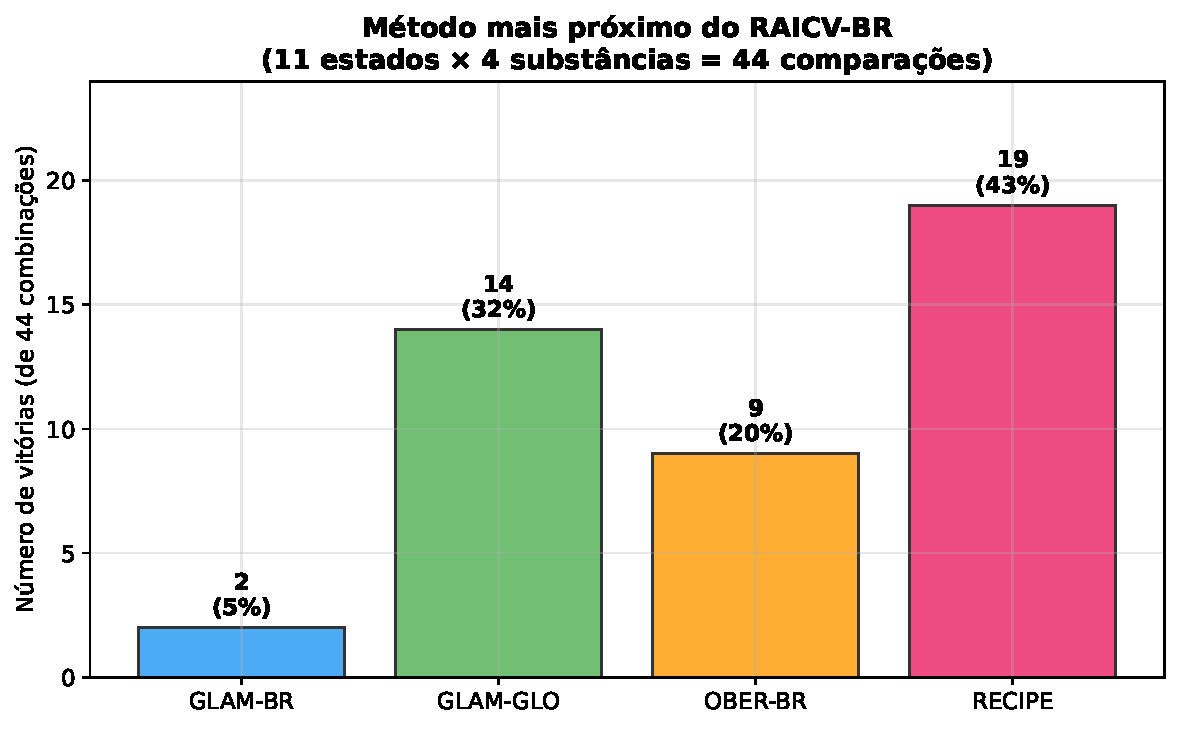
\includegraphics[width=0.75\textwidth]{figuras/fig4-vitorias-metodo.pdf}
\caption{N\'umero de combina\c{c}\~oes (estado $\times$ subst\^ancia) em que cada m\'etodo apresenta menor sMAPE em rela\c{c}\~ao ao RAICV-BR.}
\label{fig:vitorias}
\end{figure}

O ReCiPe e o GLAM-GLO s\~ao, juntos, os mais pr\'oximos do RAICV-BR em 75\% dos casos. Contudo, nenhum m\'etodo isolado \'e consistentemente superior --- a melhor alternativa depende tanto da subst\^ancia quanto do estado em an\'alise (Figura~\ref{fig:melhor-metodo}).

\begin{figure}[H]
\centering
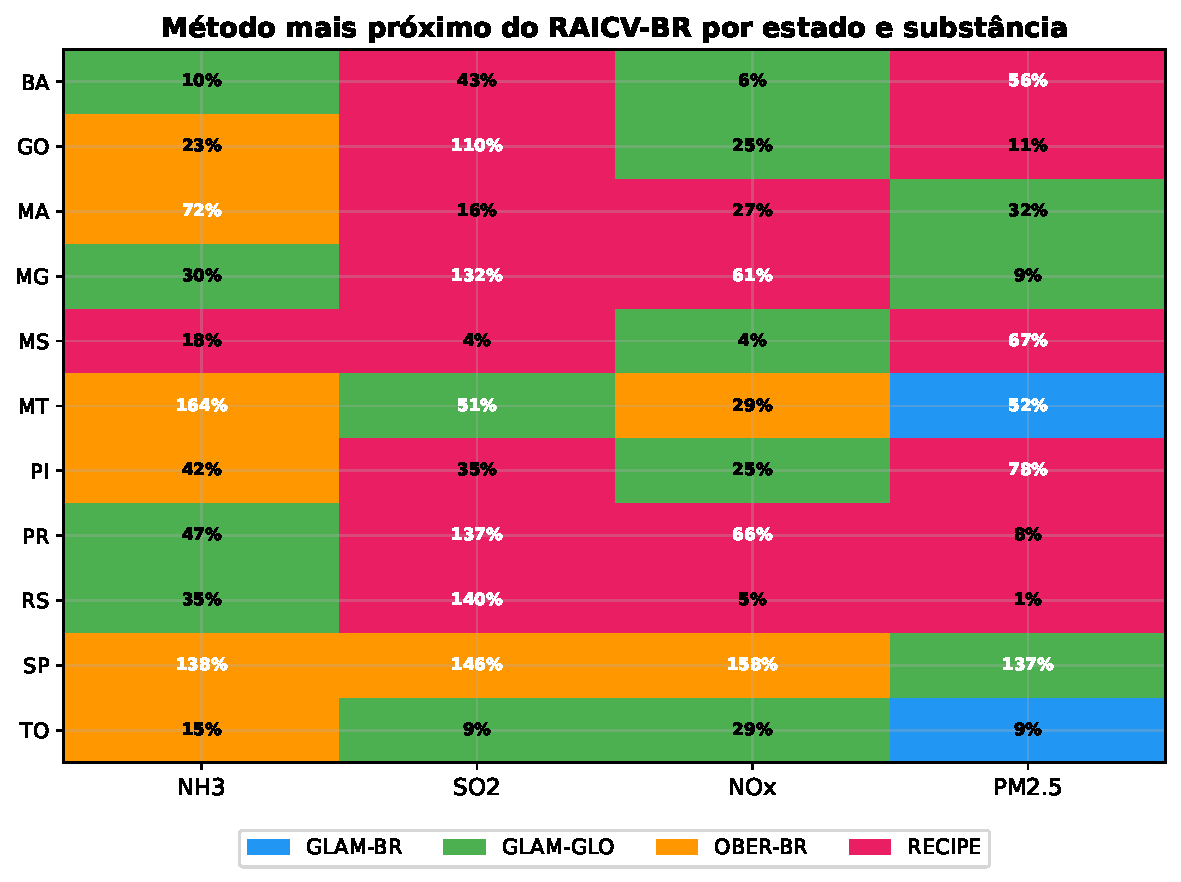
\includegraphics[width=0.85\textwidth]{figuras/fig6-mapa-melhor-metodo.pdf}
\caption{M\'etodo mais pr\'oximo do RAICV-BR por estado e subst\^ancia, com sMAPE anotado em cada c\'elula.}
\label{fig:melhor-metodo}
\end{figure}

\subsubsection{sMAPE m\'edio por m\'etodo e subst\^ancia}

A Figura~\ref{fig:barras} sumariza o sMAPE m\'edio por m\'etodo, desagregado por subst\^ancia.

\begin{figure}[H]
\centering
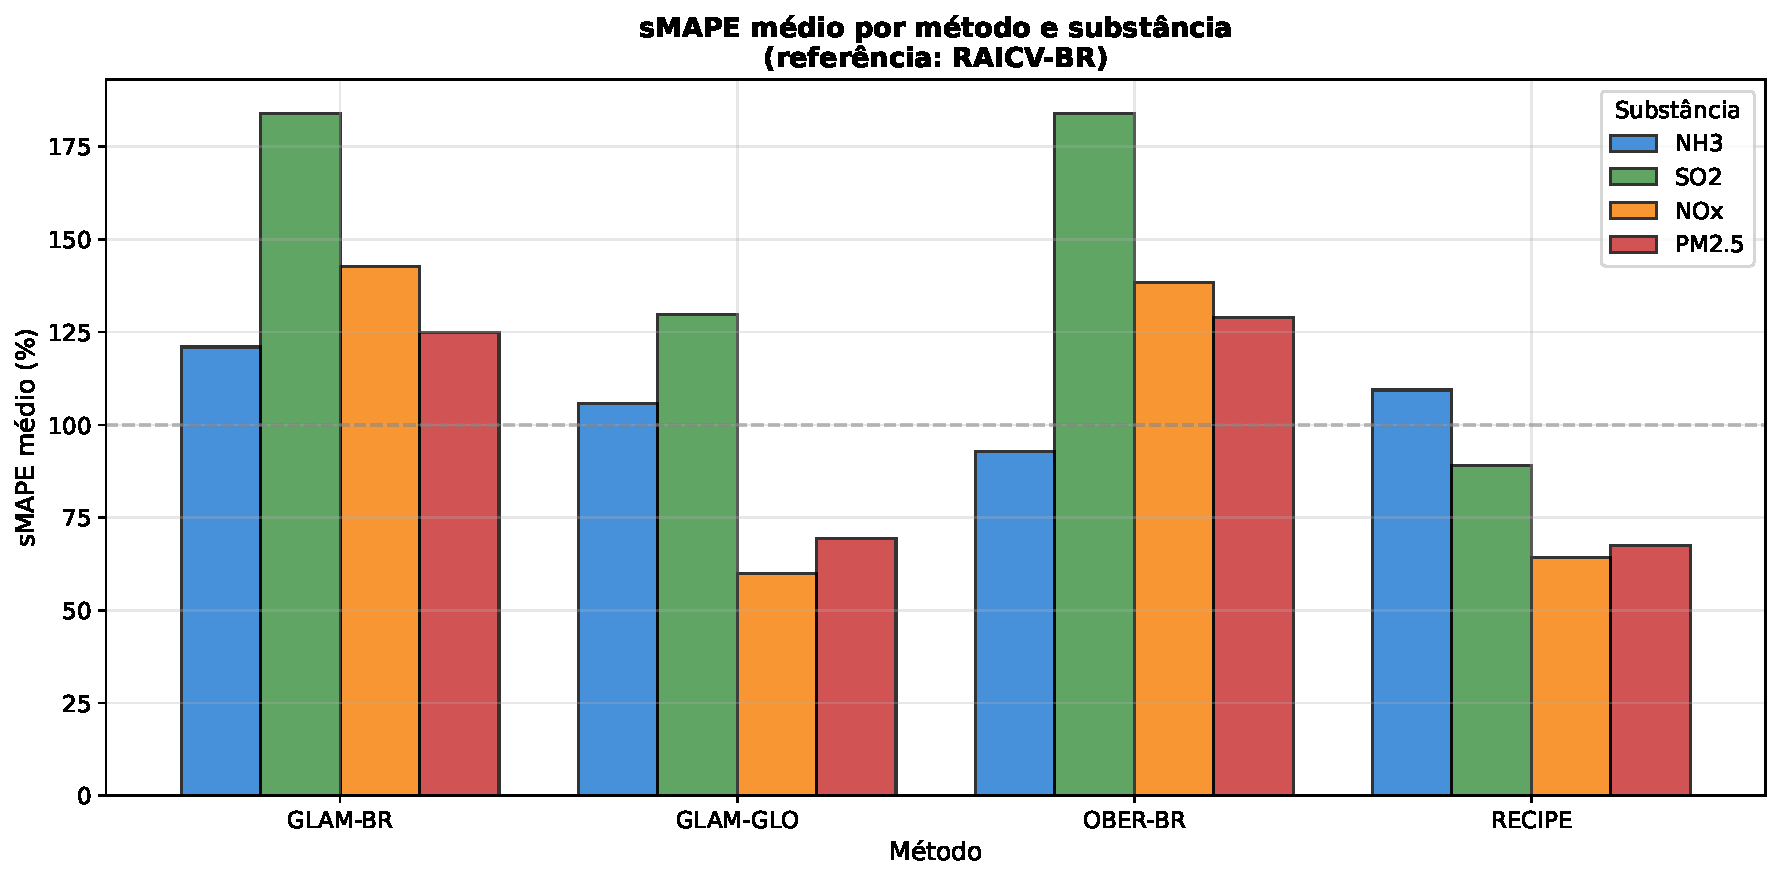
\includegraphics[width=0.85\textwidth]{figuras/fig5-barras-metodo-substancia.pdf}
\caption{sMAPE m\'edio por m\'etodo e subst\^ancia. A linha tracejada marca sMAPE = 100\%.}
\label{fig:barras}
\end{figure}

% ============================================================================
\subsection{Discuss\~ao}
% ============================================================================

Os resultados desta compara\c{c}\~ao permitem destacar cinco pontos:

\begin{enumerate}[label=\arabic*.]

\item \textbf{A escolha do m\'etodo de caracteriza\c{c}\~ao importa.} Para 3 de 4 subst\^ancias, as diferen\c{c}as entre m\'etodos s\~ao estatisticamente significativas (Kruskal-Wallis, $p < 0{,}05$). Essa sensibilidade refor\c{c}a a relev\^ancia de m\'etodos regionalizados como o RAICV-BR.

\item \textbf{Regionaliza\c{c}\~ao n\~ao implica concord\^ancia.} M\'etodos regionalizados para o Brasil (GLAM-BR, Oberschelp) n\~ao s\~ao necessariamente mais pr\'oximos do RAICV-BR do que m\'etodos globais (ReCiPe, GLAM-GLO). Cada modelo parte de premissas atmosf\'ericas, resolu\c{c}\~oes espaciais e fun\c{c}\~oes dose-resposta distintas.

\item \textbf{S\~ao Paulo \'e o caso mais cr\'itico.} Todos os m\'etodos alternativos divergem fortemente do RAICV-BR para SP (sMAPE m\'edio = 168\%), evidenciando que regi\~oes com alta complexidade urbano-industrial requerem modelagem atmosf\'erica dedicada.

\item \textbf{Nenhum m\'etodo substitui todos os outros.} O ReCiPe \'e a melhor aproxima\c{c}\~ao ao RAICV-BR em 43\% dos casos, mas em 57\% outro m\'etodo \'e mais adequado. Isso demonstra que fatores de caracteriza\c{c}\~ao contextualizados s\~ao fundamentais para estudos de ACV que pretendam refletir as condi\c{c}\~oes ambientais do Brasil.

\item \textbf{A ferramenta \texttt{olca-cf-converter} viabiliza compara\c{c}\~oes sistem\'aticas.} A capacidade de converter rapidamente diferentes conjuntos de FCs em pacotes import\'aveis pelo OpenLCA permitiu que esta compara\c{c}\~ao multim\'etodo fosse realizada de forma reprodut\'ivel e eficiente.

\end{enumerate}
